\documentclass{article}

\usepackage{fontspec}
  \setmainfont{Gentium Plus}
\usepackage{multirow}
\usepackage{tikz}
\usepackage{footnote}

\newif\ifquoteopen
\catcode`\"=\active % Allows usage of " to open and close quotes
\DeclareRobustCommand*{"}{%
   \ifquoteopen
     \quoteopenfalse ''%
   \else
     \quoteopentrue ``%
   \fi
}

\newenvironment{examples}{
  \paragraph{Examples:}
  \begin{itemize}}
  {\end{itemize}}

\title{A Descriptive Reference to Piqlau Grammar}
\author{Hank Lewis}

\begin{document}

\maketitle

\tableofcontents

\section{Abstract}

Piqlau is an SOV, head-final and primarily suffixing language with a number of unusual features, both grammatical and morphological. 
Nouns are assigned a class by the speaker, which determines its saliency and position within a clause. 
Previously introduced information, such as person and number, are often omitted, and other information, like verb tense, can be backgrounded. 
For this reason, the modern Piqlau language is highly contextual; partipants who enter conversations midway will often be at a loss without clues from the current speaker. 
Other features include a phonetic distinction between 'strong' and 'weak' vowels and frequent noun incorporation.

\section{The Speakers of the Piqlau Language}

\begin{quote}
  Long ago, innumerable worlds dotted the night sky.
  Over time, each grew reckless, forgetting the infinite hunger of the Devourer, Tawan.
  His bloodlust unsated by mortal sacrifice, he placed his great, vicious jaws upon the profligate worlds, devouring them.
  His jaws now rest on the Tawqa'in, the coral plains, and the unknown lands beyond.
  Through sacrifice alone will his thirst for blood be quenched.
\end{quote}

Or so the holy leaders of the Piqlau Empire would claim.
For hundreds of years, the Piqlau have been the Eastern continent's dominant culture, and are organized into a theocratic state centered around the appeasement of Tawan, their predator-diety.
In myth, the Tawqa'in mountains were formed long ago, when the Devourer last placed his jaws on the world.
His grip only loosened when, according to myth, the Piqlau's ancestors selflessly sent a generation to the altar, thus appeasing the god's hunger.

Piqlau culture is governed largely by religion.
Their mythos has led to a deep-seated belief that those who do not share their faith are actively furthering the world's destruction.
Subjugated peoples are commonly stripped of their culture and relegated to brutal labor before meeting their end as sacrifices.

Towns are managed by small groups of clergy, which represent a closed, hereditery caste.
With almost exclusive access to the Piqlau script, they control most written records.
The empire is centralized around Ginxu̇tu̇ and Ipaokama. These two key cities lie on opposite sides of the Great Divide, a formidible range of mountains which are impassable save for a few roads---which are treacherous and exposed.

Originally, Ginxu̇tu̇ served as the theologic and governmental capital of the entire empire, but isolation necessitated the fragmentation of power between two cities and their high-clergy.
Within the two respective halves of the Tawqa'in, mounted eunochs deliver information quickly along the empire's sophisticated road network.
In contrast, travel across the Divide is slow and often deadly.
The isolation imposed by this natural barrier has led to significant cultural differences between the two regions, akin to that of Rome and Byzantium.

No language can exist without its speakers.
The religious fervor of the Piqlau---as much as the environment in which they live and the food that they eat---defines the language presented in this grammar.
And although there is much more to the Piqlau, their practices, and their history, I will end this section here for the sake of brevity.

\section{Phonology}

\subsection{Consonants}

\begin{center}
\begin{savenotes}
\begin{tabular}{ccccc}
  Labiodental     & Alveolar & Velar      & Uvular & Glottal \\ \hline
  p b             & t d      & k          & q      & ' [ʔ]   \\
  m               & n        & g [ŋ]      &        &         \\
  \multicolumn{4}{c}{m $\sim$ n $\sim$ ŋ $\sim$ ɴ} &         \\
  f [f $\sim$ θ] & s c [ɕ] & x            &        & h\footnote{/h/ is absent in clusters and along word bounaries.}       \\
  (w)             & l        & ɭ\footnote{The velar lateral approximant only occurs in V\_V and \_\# positions.} [ʟ] w &  &        
\end{tabular}
\end{savenotes}
\end{center}

Piqlau has a modest consonant inventory, consisting of 18 consonants---although its 2 voiced stops /b d/ only occur in onset positions following nasal coda. Gemination is common in Piqlau, and can occur as a result of incorporation, compounding and the addition of suffixes\footnote{Gemination is romanized through the deduplication of the geminated phonemes letter ([al.la] > [a.lːa])}

\subsubsection{Nasal Assimilation}

When proceeding obstruents, nasal phonemes assimilate to match their place of articulation: /amsa/ $\rightarrow$ /ansa/. Voiced stops result in the nasal's complete adoption as a pre-nasal quality: /amda/ $\rightarrow$ [a.\textsuperscript{n}da].

Nasal clusters behave in the same manner, with assimilation leading to the gemination of the cluster-final nasal (<amga> /amŋa/ $\rightarrow$ <agga> [a.ŋːa]).

\subsection{Vowels}

The language features a 4-vowel inventory, which evolved from Old Piqlau's symmetrical 8 vowel system\footnote{Usually described as /a ɶ ʌ ɔ i y ɯ u/}, which featured a largely regular system of vowel harmony. 
In modern Piqlau, rounding harmony is absent outside of back vowels.

\begin{center}
\begin{savenotes}
\begin{tabular}{ccc}
  Front & \multicolumn{2}{c}{Back}                   \\ \hline
  i     & u                        & u̇ [ɯ]           \\
        & o [ɔ]                    & ȯ [ɤ $\sim$ ʌ]\footnote{Debate about the actual height of the central back unrounded vowel is ongoing; it is commonly phoneticized /ɤ/, but this can be attributed to its allophonic nature or the presence of an insufficiently studied dialectic/regional variation.}  \\
  \multicolumn{2}{c}{a $\sim$ ä}
\end{tabular}
\end{savenotes}
\end{center}

Clusters between weak vowels are broken by /h/, while all others are seperated by a glottal stop. This stop becomes weakly articulated in rapid speech /ʔ͉/, but remains phonemic. 

\subsubsection{Strong vs. Weak Quality}

Piqlau distinguishes between 'strong' and 'weak' vowels. All vowels have weak counterparts, excepting /a $\sim$ ä/, which is always weak.

\begin{center}
\begin{tabular}{cc}
  Strong       & Weak               \\ \hline
  i            & ɪ                  \\
  u ɯ          & \multirow{2}{*}{ʊ} \\    
  ɔ ɤ $\sim$ ʌ &                    \\
               & a $\sim$ ä         \\
\end{tabular}
\end{center}

The first strong vowel in a word causes other vowels that do not agree with its frontness/backness to weaken. 
As in, <iponqama> /ˈi.p\underline{ʊ}ɴ.qama/ and <tatȯpwasimi> /ta.ˈtɤ.pwa.s\underline{ɪ}.m\underline{ɪ}/, where the underlined phonemes are products of vowel weakening.

\subsubsection{Stress}

Stress falls on a word's first strong vowel. 
If none are present, it defaults to the final syllable. 
For example, <tambala> has word final stress (/tam.ba.ˈla/) because no strong vowels are present. Conversely, stress falls on the second syllable of <lapukwosan> [la.ˈpu.kwɔ.san] and the first of <xiɭambu> [ˈxi.ʟa.\textsuperscript{m}bʊ].

\subsubsection{Dipthongs}

Strong vowels do not form dipthongs. 
Dipthongs act as a single vowel in all qualities but length. 
The back dipthong /a͡ʊ/ is romanized <ao> when present in words that included a back-central vowel prior to weakening. 
This mirrors Piqlau's orthography, and distinguishes words whose roots appear identical in modern Piqlau, but whose etymologies differed in the past.

\begin{center}
\begin{tabular}{cc}
  ai [a͡ɪ] & au [a͡ʊ]
\end{tabular}
\end{center}

\subsection{Evolution from Old Piqlau}

Before the establishment of the Piqlau Empire, the Tawqa'in ranges were littered with diasporic languages---all unique, but related through Proto-Tawqa'in, an attested ancestor to modern Piqlau that introduced language to the northern reaches of the continent.

Regional dialects of the Piqlau language are numerous, but the most radical variation is between Muraiqla'u (LIT. "holy word," but hereby referred to as Clergical Piqlau) and modern Piqlau, the language's dominant dialect (often referred to by state officials as 'Low Piqlau'). 
Muraiqla'u has experienced a far more restrained series of sound changes due to the clergy's prescriptive grammar, which has been maintained and enforced by imperial scribes. 

\begin{center}
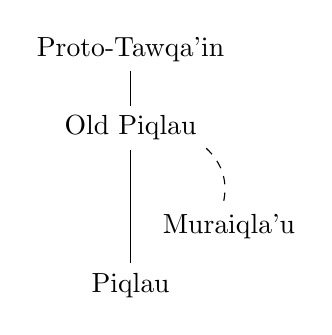
\begin{tikzpicture}
  \node (0) at (0,0) {Proto-Tawqa'in};
  \node (1) at (0,-1) {Old Piqlau};
  \node (2) at (0,-3) {Piqlau};
  \node (3) at (1.25,-2.25) {Muraiqla'u};
  \draw (0) -- (1);
  \draw (1) -- (2);
  \draw[dashed] (1) to[bend left] (3);
\end{tikzpicture}
\end{center}

With the unification of the region, Piqlau became the most prolific language in the Tawqa'in range, although many groups in the empire's extremities retained their ancestral languages\footnote{In these groups, local clergymen (almost universally the elders of the community) pass down Muraiqla'u to their successors as a second tongue, ensuring that their connection to the larger state remains intact.}
However, with the empire's bisection came generations of isolation. 
Linguistic drift slowly resulted in a sister dialect common to the Southern Empire, Kampiqlau (LIT. "valley/below language"), which is not covered in this grammar.

\begin{center}
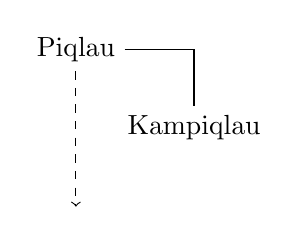
\begin{tikzpicture}
  \node (0) at (0,0) {Piqlau};
  \node (1) at (1.5,-1) {Kampiqlau};
  \draw[dashed, ->] (0) -> (0,-2);
  \draw (0) -- (1.5,0) -- (1);
\end{tikzpicture}
\end{center}

Muraiqla'u, backed with the aformentioned perscriptive grammar, did not suffer the same variation. 
The language's orthography was developed by members of the theocracy and thus was tailored to the Clergical tongue.

\subsubsection{Survey of the Parent Language}

Old Piqlau's inventory was much larger than its modern descendent.
Among other phonemes, Old Piqlau included a complete uvular series, a rhotic tap, and a voiced labial fricative. 
Its vowel system obeyed strict rounding harmony. 

Over time, the distinctions between many phonemes gradually degraded, while other sounds were simply lost, resulting in the language's current form.

\begin{center}
\begin{tabular}{cccccc}
  Labial & Dental    & Alveolar            & Velar & Uvular & Glottal \\ \hline
  p b    & \multicolumn{2}{c}{t d}         & k g   & q ɢ    & ʔ       \\
  m      & \multicolumn{2}{c}{n̪ $\sim$ n}  & ŋ     & ɴ      &         \\
  ɸ $\sim$ f β $\sim$ v & θ & s            & x     & χ      &         \\
  (w)    &           & l $\sim$ ɹ ɾ        & w ʟ   &        &        
\end{tabular}
\end{center}

\begin{center}
\begin{tabular}{cc}
  Front & Back       \\ \hline
  i y   & ɯ u          \\
  a ɶ   & ɤ $\sim$ ʌ ɔ \\
\end{tabular}
\end{center}

Syllables in Old Piqlau always began with a non-approximant consonant and, optionally, ended in a sonorant. 
Its syllable structure is best defined as CV(S)\footnote{Although some exceptions have been observed. See footnotes to Section 3.1.}. 
However, as a result of sound changes, the modern language's structure looks significantly different. 
Stress was almost universally word-initial, although speakers from certain regions would avoid placing stress on syllables with the nuclei /a ɶ/.

\subsubsection{Sound Changes \& Allophony}

This section documents a reconstructed series of sound changes that distinguish modern Piqlau from its parent language. The most significant changes documented are the loss of rounding harmony and the acquisition of modern Piqlau's unusual distinction in vowel strength.

\begin{itemize}
  \item /ɢ ɴ χ/ $\rightarrow$ /g ŋ x/
  \item /b/ $\rightarrow$ /β $\sim$ v/ V\_V
  \item /b d g/ $\rightarrow$ /p t k/ [C][-nasal]\_
  \item Approximant-Obstruent clusters metathesize (e.g. /aw.ko/ $\rightarrow$ /a.kwo/)
  \item /β $\sim$ v/ $\rightarrow$ /ɸ $\sim$ f/
  \item /ɸ $\sim$ f/ $\rightarrow$ /f/ \& /f/ becomes indistinct from dental fricative /θ/ (/f $\sim$ θ/)
  \item Rounding harmony gradually lost, except in back vowels
  \begin{item}
    Distinction between strong \& weak vowels emerges\footnote{See Section 3.2.1.}

    \subitem /i/ $\rightarrow$ /ɪ/ when word contains stressed back vowel
    \subitem /u ɯ ɔ ɤ $\sim$ ʌ/ $\rightarrow$ /ʊ/ when word contains /ˈi/
  \end{item}
  \item /ʔ/ $\rightarrow$ /h/ between weak vowels
  \item /h/ $\rightarrow$ ∅ a\_ɪ a\_ʊ \& /aɪ aʊ/ $\rightarrow$ /a͡ɪ a͡ʊ/
  \item /ɾ/ $\rightarrow$ /l $\sim$ ɹ/\footnote{In modern Piqlau, /l/ is legal in \#\_ positions as a result of this sound change.}
  \item /ʟ/ $\rightarrow$ /l $\sim$ ɹ/ \_[C][-nasal]
  \item /s/ $\rightarrow$ /ɕ/ \_C
  \item /ŋg/ $\rightarrow$ /ŋː/\footnote{Although the gemination of the velar nasal is contested, it appears that /g/ is lost following nasals, while /b d/ remain under equivalent circumstances.}
\end{itemize}

\subsection{Phonotactics}

Modern Piqlau's syllable structure is best described as CV(C).

Only a small number of consonant clusters can be attested; all others are considered inviolate of the language's phonotactics.

\subsubsection{Legal Consonant Clusters}

Although Old Piqlau only permitted sonorant coda, the current language permits a specific set of obstruent coda---but only when the following onset is compatible. 
The irregularity of Piqlau's cluster constraints is a product of its historical sound changes\footnote{See Section 3.2.2.}.

\begin{center}
\begin{savenotes}
\footnotesize
\begin{tabular}{c | cccccccccccccc}
    & \multirow{2}{*}{m} & \multirow{2}{*}{n} & g & n\footnote{Not phonemic; only occurs before /q/ as a result of nasal assimilation. Romanized in the same manner as the dento-alveolar nasal /n/.} & \multirow{2}{*}{w} & \multirow{2}{*}{l} & ɭ & \multirow{2}{*}{p} & \multirow{2}{*}{t} & \multirow{2}{*}{k} & \multirow{2}{*}{q} & \multirow{2}{*}{f} & sh & \multirow{2}{*}{x} \\
    & & & [ŋ] & [ɴ] & & & [ʟ] & & & & & & [ɕ] & \\ \hline
  p & mp & & & & & & & & & & & & & \\
  b & mb & & & & & & & & & & & & & \\
  t & & nt & & & & & & & & & & & & \\
  d & & nd & & & & & & & & & & & & \\
  k & & & gk & & & & & & & & & & & \\
  q & & & & nq & & & & & & & & & & \\
  f & mf\footnote{The cluster-initial nasal varies according to the speaker's realization of /f $\sim$ θ/. If the fricative is dentalized, the preceeding nasal becomes /n̪/.} & & & & & & & & & & & & & \\
  s & & ns & & & & & & & & & & & & \\
  x & & & gx & & & & & & & & & & & \\
  m & mm & & & & wm & lm & ɭm & & & & & & & \\
  n & & nn & & & wn & ln & ɭn & & & & & & & \\
  g [ŋ] & & & gg & & wg & lg & ɭg & & & & & & & \\
  w & mw & nw & gw & & ww & & & pw & tw & kw & qw & fw & shw & xw \\
  l & ml & nl & gl & & wl & ll & & pl & tl & kl & ql & fl & shl & xl \\
\end{tabular}
\end{savenotes}
\end{center}

\end{document}